\documentclass{whiteboard}
\begin{document}
\begin{frame}[plain,t]
\bbcover{OJ 10600}{ACM contest and Blackout}{Prof. Edson Alves}{Faculdade UnB Gama}

\end{frame}
\begin{frame}[plain,t]
\vspace*{\fill}

\bbenglish{In order to prepare the “The First National ACM School Contest” (in 20??) the major of the city decided to provide all the schools with a reliable source of power (The major is really afraid of blackouts).  So, in order to do that, power station ``Future'' and one school (doesn’t matter which one) must be connected; in addition, some schools must be connected as well.}

\vspace{0.1in}

\bbenglish{You may assume that a school has a reliable source of power if it’s connected directly to ``Future'', or to any other school that has a reliable source of power. You are given the cost of connection between some schools. The major has decided to pick out two the cheapest connection plans – the cost of the connection is equal to the sum of the connections between the schools. Your task is to help the major -- find the cost of the two cheapest connection plans.}

\vspace*{\fill}
\end{frame}
\begin{frame}[plain,t]
\vspace*{\fill}

\bbtext{Durante os preparativos da “Primeira Maratona Nacional Escolar ACM" (em 20??), o prefeito da cidade decidiu prover todas as escolas com uma fonte de energia confiável (na verdade o prefeito está preocupado com blecautes).  Assim, para atingir este objetivo, a estação de energia ``Futuro'' e uma escola (não importa qual) devem estar conectadas; além disso, algumas outras escolas devem estar conectadas também.}

\vspace{0.1in}

\bbtext{Você pode assumir que uma escola tem uma fonte de energia confiável se ela está conectada diratamente a ``Futuro'', ou a qualquer escola que tenha uma fonte de energia confiável. Serão dados os custos de conexão entre algumas escolas. O prefeito tem que decidir entre os dois planos de conexão mais baratos -- o custo de conexão é igual a soma das conexões entre todas as escolas. Sua tarefa é ajudar o prefeito -- determine os custos dos dois planos mais baratos.}

\vspace*{\fill}
\end{frame}
\begin{frame}[plain,t]
\vspace*{\fill}

\bbbold{Input}

\vspace{0.1in}

\bbenglish{The Input starts with the number of test cases, $T$ $(1 < T < 15)$ on a line. Then $T$ test cases follow. The first line of every test case contains two numbers, which are separated by a space, $N$ $(3 < N < 100)$ the number of schools in the city, and $M$ the number of possible connections among them. Next $M$ lines contain three numbers $A_i, B_i, C_i$, where $C_i$ is the cost of the connection $(1 < C_i < 300)$ between schools $A_i$ and $B_i$. The schools are numbered with integers in the range $1$ to $N$.}

\vspace{0.2in}

\bbbold{Output}

\vspace{0.1in}

\bbenglish{For every test case print only one line of output. This line should contain two numbers separated by a single space -- the cost of two the cheapest connection plans. Let $S_1$ be the cheapest cost and $S_2$ the next cheapest cost. It’s important, that $S_1 = S_2$ if and only if there are two cheapest plans, otherwise $S_1 < S_2$. You can assume that it is always possible to find the costs $S_1$ and $S_2$.}

\vspace*{\fill}
\end{frame}
\begin{frame}[plain,t]
\vspace*{\fill}

\bbbold{Entrada}

\vspace{0.1in}

\bbtext{A entrada começa com o número de casos de teste $T$ $(1 < T < 15)$ em uma linha. Então seguem $T$ casos de teste. A primeira linha de cada caso de teste contém dois inteiros, separados por um espaço em branco, $N$ $(3 < N < 100)$, o número de escolas na cidade, e $M$, o número de conexões possíveis entre elas. As próximas $M$ linhas contém três números $A_i, B_i, C_i$, onde $C_i$ é o custo da conexão $(1 < C_i < 300)$ entre as escolas $A_i$ e $B_i$. As escolas estão numeradas com inteiros de $1$ a $N$.}

\vspace{0.2in}

\bbbold{Saída}

\vspace{0.1in}

\bbtext{Para cada caso de teste imprima uma única linha. Esta linha deverá conter dois inteiros separados por um único espaço -- o custo dos dois planos de conexão mais baratos. Seja $S_1$ o custo do plano mais barato e $S_2$ o custo do segundo plano mais barato. Imporante: $S_1 = S_2$ se e somente se há dois planos mais baratos, caso contrário $S_1 < S_2$. Você pode assumir que é sempre possível encontrar os custos $S_1$ e $S_2$.}

\vspace*{\fill}
\end{frame}
\begin{frame}[plain,t]
\begin{tikzpicture}
\node[draw,opacity=0] at (0, 0) {x};
\node[draw,opacity=0] at (14, 8) {x};

	\node[anchor=west] (header) at (0, 7.0) { \bbbold{Exemplo de entrada e saída} };

\end{tikzpicture}
\end{frame}
\begin{frame}[plain,t]
\begin{tikzpicture}
\node[draw,opacity=0] at (0, 0) {x};
\node[draw,opacity=0] at (14, 8) {x};

	\node[anchor=west] (header) at (0, 7.0) { \bbbold{Exemplo de entrada e saída} };


	\node[anchor=west] (line1) at (1.0, 6.0) { \bbtext{\texttt{5 8} } };

\end{tikzpicture}
\end{frame}
\begin{frame}[plain,t]
\begin{tikzpicture}
\node[draw,opacity=0] at (0, 0) {x};
\node[draw,opacity=0] at (14, 8) {x};

	\node[anchor=west] (header) at (0, 7.0) { \bbbold{Exemplo de entrada e saída} };


	\node[anchor=west] (line1) at (1.0, 6.0) { \bbtext{\texttt{5 8} } };


	\draw[->,color=BBViolet] (1.25, 5.0) to  (1.25, 5.75);

	\node[] (r) at (1.25, 4.75) { \footnotesize \bbcomment{\# de escolas} };

\end{tikzpicture}
\end{frame}
\begin{frame}[plain,t]
\begin{tikzpicture}
\node[draw,opacity=0] at (0, 0) {x};
\node[draw,opacity=0] at (14, 8) {x};

	\node[anchor=west] (header) at (0, 7.0) { \bbbold{Exemplo de entrada e saída} };


	\node[anchor=west] (line1) at (1.0, 6.0) { \bbtext{\texttt{5 8} } };


	\draw[->,color=BBViolet] (1.65, 5.0) to  (1.65, 5.75);

	\node[] (r) at (1.65, 4.75) { \footnotesize \bbcomment{\# de conexões} };



\end{tikzpicture}
\end{frame}
\begin{frame}[plain,t]
\begin{tikzpicture}
\node[draw,opacity=0] at (0, 0) {x};
\node[draw,opacity=0] at (14, 8) {x};

	\node[anchor=west] (header) at (0, 7.0) { \bbbold{Exemplo de entrada e saída} };


	\node[anchor=west] (line1) at (1.0, 6.0) { \bbtext{\texttt{5 8} } };








	\node[draw,very thick,circle] (node1) at (7.0, 4.5) { \bbtext{1} };

	\node[draw,very thick,circle] (node2) at (10.0, 7.0) { \bbtext{2} };

	\node[draw,very thick,circle] (node3) at (13.0, 4.5) { \bbtext{3} };

	\node[draw,very thick,circle] (node4) at (13.0, 1.0) { \bbtext{4} };

	\node[draw,very thick,circle] (node5) at (7.0, 1.0) { \bbtext{5} };

\end{tikzpicture}
\end{frame}
\begin{frame}[plain,t]
\begin{tikzpicture}
\node[draw,opacity=0] at (0, 0) {x};
\node[draw,opacity=0] at (14, 8) {x};

	\node[anchor=west] (header) at (0, 7.0) { \bbbold{Exemplo de entrada e saída} };


	\node[anchor=west] (line1) at (1.0, 6.0) { \bbtext{\texttt{5 8} } };








	\node[draw,very thick,circle] (node1) at (7.0, 4.5) { \bbtext{1} };

	\node[draw,very thick,circle] (node2) at (10.0, 7.0) { \bbtext{2} };

	\node[draw,very thick,circle] (node3) at (13.0, 4.5) { \bbtext{3} };

	\node[draw,very thick,circle] (node4) at (13.0, 1.0) { \bbtext{4} };

	\node[draw,very thick,circle] (node5) at (7.0, 1.0) { \bbtext{5} };


	\node[anchor=west] (line2) at (1.0, 5.5) { \bbtext{\texttt{1 3 75} } };

\end{tikzpicture}
\end{frame}
\begin{frame}[plain,t]
\begin{tikzpicture}
\node[draw,opacity=0] at (0, 0) {x};
\node[draw,opacity=0] at (14, 8) {x};

	\node[anchor=west] (header) at (0, 7.0) { \bbbold{Exemplo de entrada e saída} };


	\node[anchor=west] (line1) at (1.0, 6.0) { \bbtext{\texttt{5 8} } };


	\draw[->,color=BBViolet] (1.25, 5.25) to  (1.25, 4.25);

	\node[] (r) at (1.25, 4.0) { \footnotesize \bbcomment{cidade A} };





	\node[draw,very thick,circle] (node1) at (7.0, 4.5) { \bbtext{1} };

	\node[draw,very thick,circle] (node2) at (10.0, 7.0) { \bbtext{2} };

	\node[draw,very thick,circle] (node3) at (13.0, 4.5) { \bbtext{3} };

	\node[draw,very thick,circle] (node4) at (13.0, 1.0) { \bbtext{4} };

	\node[draw,very thick,circle] (node5) at (7.0, 1.0) { \bbtext{5} };


	\node[anchor=west] (line2) at (1.0, 5.5) { \bbtext{\texttt{1 3 75} } };




\end{tikzpicture}
\end{frame}
\begin{frame}[plain,t]
\begin{tikzpicture}
\node[draw,opacity=0] at (0, 0) {x};
\node[draw,opacity=0] at (14, 8) {x};

	\node[anchor=west] (header) at (0, 7.0) { \bbbold{Exemplo de entrada e saída} };


	\node[anchor=west] (line1) at (1.0, 6.0) { \bbtext{\texttt{5 8} } };


	\draw[->,color=BBViolet] (1.65, 5.25) to  (1.65, 4.25);

	\node[] (r) at (1.65, 4.0) { \footnotesize \bbcomment{cidade B} };





	\node[draw,very thick,circle] (node1) at (7.0, 4.5) { \bbtext{1} };

	\node[draw,very thick,circle] (node2) at (10.0, 7.0) { \bbtext{2} };

	\node[draw,very thick,circle] (node3) at (13.0, 4.5) { \bbtext{3} };

	\node[draw,very thick,circle] (node4) at (13.0, 1.0) { \bbtext{4} };

	\node[draw,very thick,circle] (node5) at (7.0, 1.0) { \bbtext{5} };


	\node[anchor=west] (line2) at (1.0, 5.5) { \bbtext{\texttt{1 3 75} } };







\end{tikzpicture}
\end{frame}
\begin{frame}[plain,t]
\begin{tikzpicture}
\node[draw,opacity=0] at (0, 0) {x};
\node[draw,opacity=0] at (14, 8) {x};

	\node[anchor=west] (header) at (0, 7.0) { \bbbold{Exemplo de entrada e saída} };


	\node[anchor=west] (line1) at (1.0, 6.0) { \bbtext{\texttt{5 8} } };


	\draw[->,color=BBViolet] (2.15, 5.25) to  (2.15, 4.25);

	\node[] (r) at (2.15, 4.0) { \footnotesize \bbcomment{custo} };





	\node[draw,very thick,circle] (node1) at (7.0, 4.5) { \bbtext{1} };

	\node[draw,very thick,circle] (node2) at (10.0, 7.0) { \bbtext{2} };

	\node[draw,very thick,circle] (node3) at (13.0, 4.5) { \bbtext{3} };

	\node[draw,very thick,circle] (node4) at (13.0, 1.0) { \bbtext{4} };

	\node[draw,very thick,circle] (node5) at (7.0, 1.0) { \bbtext{5} };


	\node[anchor=west] (line2) at (1.0, 5.5) { \bbtext{\texttt{1 3 75} } };










\end{tikzpicture}
\end{frame}
\begin{frame}[plain,t]
\begin{tikzpicture}
\node[draw,opacity=0] at (0, 0) {x};
\node[draw,opacity=0] at (14, 8) {x};

	\node[anchor=west] (header) at (0, 7.0) { \bbbold{Exemplo de entrada e saída} };


	\node[anchor=west] (line1) at (1.0, 6.0) { \bbtext{\texttt{5 8} } };








	\node[draw,very thick,circle] (node1) at (7.0, 4.5) { \bbtext{1} };

	\node[draw,very thick,circle] (node2) at (10.0, 7.0) { \bbtext{2} };

	\node[draw,very thick,circle] (node3) at (13.0, 4.5) { \bbtext{3} };

	\node[draw,very thick,circle] (node4) at (13.0, 1.0) { \bbtext{4} };

	\node[draw,very thick,circle] (node5) at (7.0, 1.0) { \bbtext{5} };


	\node[anchor=west] (line2) at (1.0, 5.5) { \bbtext{\texttt{1 3 75} } };












	\draw[thick](node1) to node[above] { \footnotesize \bbinfo{75} } (node3);

\end{tikzpicture}
\end{frame}
\begin{frame}[plain,t]
\begin{tikzpicture}
\node[draw,opacity=0] at (0, 0) {x};
\node[draw,opacity=0] at (14, 8) {x};

	\node[anchor=west] (header) at (0, 7.0) { \bbbold{Exemplo de entrada e saída} };


	\node[anchor=west] (line1) at (1.0, 6.0) { \bbtext{\texttt{5 8} } };








	\node[draw,very thick,circle] (node1) at (7.0, 4.5) { \bbtext{1} };

	\node[draw,very thick,circle] (node2) at (10.0, 7.0) { \bbtext{2} };

	\node[draw,very thick,circle] (node3) at (13.0, 4.5) { \bbtext{3} };

	\node[draw,very thick,circle] (node4) at (13.0, 1.0) { \bbtext{4} };

	\node[draw,very thick,circle] (node5) at (7.0, 1.0) { \bbtext{5} };


	\node[anchor=west] (line2) at (1.0, 5.5) { \bbtext{\texttt{1 3 75} } };












	\draw[thick](node1) to node[above] { \footnotesize \bbinfo{75} } (node3);


	\node[anchor=west] (line3) at (1.0, 5.0) { \bbtext{\texttt{3 4 51} } };

\end{tikzpicture}
\end{frame}
\begin{frame}[plain,t]
\begin{tikzpicture}
\node[draw,opacity=0] at (0, 0) {x};
\node[draw,opacity=0] at (14, 8) {x};

	\node[anchor=west] (header) at (0, 7.0) { \bbbold{Exemplo de entrada e saída} };


	\node[anchor=west] (line1) at (1.0, 6.0) { \bbtext{\texttt{5 8} } };








	\node[draw,very thick,circle] (node1) at (7.0, 4.5) { \bbtext{1} };

	\node[draw,very thick,circle] (node2) at (10.0, 7.0) { \bbtext{2} };

	\node[draw,very thick,circle] (node3) at (13.0, 4.5) { \bbtext{3} };

	\node[draw,very thick,circle] (node4) at (13.0, 1.0) { \bbtext{4} };

	\node[draw,very thick,circle] (node5) at (7.0, 1.0) { \bbtext{5} };


	\node[anchor=west] (line2) at (1.0, 5.5) { \bbtext{\texttt{1 3 75} } };












	\draw[thick](node1) to node[above] { \footnotesize \bbinfo{75} } (node3);


	\node[anchor=west] (line3) at (1.0, 5.0) { \bbtext{\texttt{3 4 51} } };


	\draw[thick](node3) to node[right] { \footnotesize \bbinfo{51} } (node4);

\end{tikzpicture}
\end{frame}
\begin{frame}[plain,t]
\begin{tikzpicture}
\node[draw,opacity=0] at (0, 0) {x};
\node[draw,opacity=0] at (14, 8) {x};

	\node[anchor=west] (header) at (0, 7.0) { \bbbold{Exemplo de entrada e saída} };


	\node[anchor=west] (line1) at (1.0, 6.0) { \bbtext{\texttt{5 8} } };








	\node[draw,very thick,circle] (node1) at (7.0, 4.5) { \bbtext{1} };

	\node[draw,very thick,circle] (node2) at (10.0, 7.0) { \bbtext{2} };

	\node[draw,very thick,circle] (node3) at (13.0, 4.5) { \bbtext{3} };

	\node[draw,very thick,circle] (node4) at (13.0, 1.0) { \bbtext{4} };

	\node[draw,very thick,circle] (node5) at (7.0, 1.0) { \bbtext{5} };


	\node[anchor=west] (line2) at (1.0, 5.5) { \bbtext{\texttt{1 3 75} } };












	\draw[thick](node1) to node[above] { \footnotesize \bbinfo{75} } (node3);


	\node[anchor=west] (line3) at (1.0, 5.0) { \bbtext{\texttt{3 4 51} } };


	\draw[thick](node3) to node[right] { \footnotesize \bbinfo{51} } (node4);


	\node[anchor=west] (line4) at (1.0, 4.5) { \bbtext{\texttt{2 4 19} } };

\end{tikzpicture}
\end{frame}
\begin{frame}[plain,t]
\begin{tikzpicture}
\node[draw,opacity=0] at (0, 0) {x};
\node[draw,opacity=0] at (14, 8) {x};

	\node[anchor=west] (header) at (0, 7.0) { \bbbold{Exemplo de entrada e saída} };


	\node[anchor=west] (line1) at (1.0, 6.0) { \bbtext{\texttt{5 8} } };








	\node[draw,very thick,circle] (node1) at (7.0, 4.5) { \bbtext{1} };

	\node[draw,very thick,circle] (node2) at (10.0, 7.0) { \bbtext{2} };

	\node[draw,very thick,circle] (node3) at (13.0, 4.5) { \bbtext{3} };

	\node[draw,very thick,circle] (node4) at (13.0, 1.0) { \bbtext{4} };

	\node[draw,very thick,circle] (node5) at (7.0, 1.0) { \bbtext{5} };


	\node[anchor=west] (line2) at (1.0, 5.5) { \bbtext{\texttt{1 3 75} } };












	\draw[thick](node1) to node[above] { \footnotesize \bbinfo{75} } (node3);


	\node[anchor=west] (line3) at (1.0, 5.0) { \bbtext{\texttt{3 4 51} } };


	\draw[thick](node3) to node[right] { \footnotesize \bbinfo{51} } (node4);


	\node[anchor=west] (line4) at (1.0, 4.5) { \bbtext{\texttt{2 4 19} } };


	\draw[thick](node2) to node[above right,pos=0.7] { \footnotesize \bbinfo{19} } (node4);

\end{tikzpicture}
\end{frame}
\begin{frame}[plain,t]
\begin{tikzpicture}
\node[draw,opacity=0] at (0, 0) {x};
\node[draw,opacity=0] at (14, 8) {x};

	\node[anchor=west] (header) at (0, 7.0) { \bbbold{Exemplo de entrada e saída} };


	\node[anchor=west] (line1) at (1.0, 6.0) { \bbtext{\texttt{5 8} } };








	\node[draw,very thick,circle] (node1) at (7.0, 4.5) { \bbtext{1} };

	\node[draw,very thick,circle] (node2) at (10.0, 7.0) { \bbtext{2} };

	\node[draw,very thick,circle] (node3) at (13.0, 4.5) { \bbtext{3} };

	\node[draw,very thick,circle] (node4) at (13.0, 1.0) { \bbtext{4} };

	\node[draw,very thick,circle] (node5) at (7.0, 1.0) { \bbtext{5} };


	\node[anchor=west] (line2) at (1.0, 5.5) { \bbtext{\texttt{1 3 75} } };












	\draw[thick](node1) to node[above] { \footnotesize \bbinfo{75} } (node3);


	\node[anchor=west] (line3) at (1.0, 5.0) { \bbtext{\texttt{3 4 51} } };


	\draw[thick](node3) to node[right] { \footnotesize \bbinfo{51} } (node4);


	\node[anchor=west] (line4) at (1.0, 4.5) { \bbtext{\texttt{2 4 19} } };


	\draw[thick](node2) to node[above right,pos=0.7] { \footnotesize \bbinfo{19} } (node4);


	\node[anchor=west] (line5) at (1.0, 4.0) { \bbtext{\texttt{3 2 95} } };

\end{tikzpicture}
\end{frame}
\begin{frame}[plain,t]
\begin{tikzpicture}
\node[draw,opacity=0] at (0, 0) {x};
\node[draw,opacity=0] at (14, 8) {x};

	\node[anchor=west] (header) at (0, 7.0) { \bbbold{Exemplo de entrada e saída} };


	\node[anchor=west] (line1) at (1.0, 6.0) { \bbtext{\texttt{5 8} } };








	\node[draw,very thick,circle] (node1) at (7.0, 4.5) { \bbtext{1} };

	\node[draw,very thick,circle] (node2) at (10.0, 7.0) { \bbtext{2} };

	\node[draw,very thick,circle] (node3) at (13.0, 4.5) { \bbtext{3} };

	\node[draw,very thick,circle] (node4) at (13.0, 1.0) { \bbtext{4} };

	\node[draw,very thick,circle] (node5) at (7.0, 1.0) { \bbtext{5} };


	\node[anchor=west] (line2) at (1.0, 5.5) { \bbtext{\texttt{1 3 75} } };












	\draw[thick](node1) to node[above] { \footnotesize \bbinfo{75} } (node3);


	\node[anchor=west] (line3) at (1.0, 5.0) { \bbtext{\texttt{3 4 51} } };


	\draw[thick](node3) to node[right] { \footnotesize \bbinfo{51} } (node4);


	\node[anchor=west] (line4) at (1.0, 4.5) { \bbtext{\texttt{2 4 19} } };


	\draw[thick](node2) to node[above right,pos=0.7] { \footnotesize \bbinfo{19} } (node4);


	\node[anchor=west] (line5) at (1.0, 4.0) { \bbtext{\texttt{3 2 95} } };


	\draw[thick](node3) to node[above right] { \footnotesize \bbinfo{95} } (node2);

\end{tikzpicture}
\end{frame}
\begin{frame}[plain,t]
\begin{tikzpicture}
\node[draw,opacity=0] at (0, 0) {x};
\node[draw,opacity=0] at (14, 8) {x};

	\node[anchor=west] (header) at (0, 7.0) { \bbbold{Exemplo de entrada e saída} };


	\node[anchor=west] (line1) at (1.0, 6.0) { \bbtext{\texttt{5 8} } };








	\node[draw,very thick,circle] (node1) at (7.0, 4.5) { \bbtext{1} };

	\node[draw,very thick,circle] (node2) at (10.0, 7.0) { \bbtext{2} };

	\node[draw,very thick,circle] (node3) at (13.0, 4.5) { \bbtext{3} };

	\node[draw,very thick,circle] (node4) at (13.0, 1.0) { \bbtext{4} };

	\node[draw,very thick,circle] (node5) at (7.0, 1.0) { \bbtext{5} };


	\node[anchor=west] (line2) at (1.0, 5.5) { \bbtext{\texttt{1 3 75} } };












	\draw[thick](node1) to node[above] { \footnotesize \bbinfo{75} } (node3);


	\node[anchor=west] (line3) at (1.0, 5.0) { \bbtext{\texttt{3 4 51} } };


	\draw[thick](node3) to node[right] { \footnotesize \bbinfo{51} } (node4);


	\node[anchor=west] (line4) at (1.0, 4.5) { \bbtext{\texttt{2 4 19} } };


	\draw[thick](node2) to node[above right,pos=0.7] { \footnotesize \bbinfo{19} } (node4);


	\node[anchor=west] (line5) at (1.0, 4.0) { \bbtext{\texttt{3 2 95} } };


	\draw[thick](node3) to node[above right] { \footnotesize \bbinfo{95} } (node2);


	\node[anchor=west] (line6) at (1.0, 3.5) { \bbtext{\texttt{2 5 42} } };

\end{tikzpicture}
\end{frame}
\begin{frame}[plain,t]
\begin{tikzpicture}
\node[draw,opacity=0] at (0, 0) {x};
\node[draw,opacity=0] at (14, 8) {x};

	\node[anchor=west] (header) at (0, 7.0) { \bbbold{Exemplo de entrada e saída} };


	\node[anchor=west] (line1) at (1.0, 6.0) { \bbtext{\texttt{5 8} } };








	\node[draw,very thick,circle] (node1) at (7.0, 4.5) { \bbtext{1} };

	\node[draw,very thick,circle] (node2) at (10.0, 7.0) { \bbtext{2} };

	\node[draw,very thick,circle] (node3) at (13.0, 4.5) { \bbtext{3} };

	\node[draw,very thick,circle] (node4) at (13.0, 1.0) { \bbtext{4} };

	\node[draw,very thick,circle] (node5) at (7.0, 1.0) { \bbtext{5} };


	\node[anchor=west] (line2) at (1.0, 5.5) { \bbtext{\texttt{1 3 75} } };












	\draw[thick](node1) to node[above] { \footnotesize \bbinfo{75} } (node3);


	\node[anchor=west] (line3) at (1.0, 5.0) { \bbtext{\texttt{3 4 51} } };


	\draw[thick](node3) to node[right] { \footnotesize \bbinfo{51} } (node4);


	\node[anchor=west] (line4) at (1.0, 4.5) { \bbtext{\texttt{2 4 19} } };


	\draw[thick](node2) to node[above right,pos=0.7] { \footnotesize \bbinfo{19} } (node4);


	\node[anchor=west] (line5) at (1.0, 4.0) { \bbtext{\texttt{3 2 95} } };


	\draw[thick](node3) to node[above right] { \footnotesize \bbinfo{95} } (node2);


	\node[anchor=west] (line6) at (1.0, 3.5) { \bbtext{\texttt{2 5 42} } };


	\draw[thick](node2) to node[above left,pos=0.7] { \footnotesize \bbinfo{42} } (node5);

\end{tikzpicture}
\end{frame}
\begin{frame}[plain,t]
\begin{tikzpicture}
\node[draw,opacity=0] at (0, 0) {x};
\node[draw,opacity=0] at (14, 8) {x};

	\node[anchor=west] (header) at (0, 7.0) { \bbbold{Exemplo de entrada e saída} };


	\node[anchor=west] (line1) at (1.0, 6.0) { \bbtext{\texttt{5 8} } };








	\node[draw,very thick,circle] (node1) at (7.0, 4.5) { \bbtext{1} };

	\node[draw,very thick,circle] (node2) at (10.0, 7.0) { \bbtext{2} };

	\node[draw,very thick,circle] (node3) at (13.0, 4.5) { \bbtext{3} };

	\node[draw,very thick,circle] (node4) at (13.0, 1.0) { \bbtext{4} };

	\node[draw,very thick,circle] (node5) at (7.0, 1.0) { \bbtext{5} };


	\node[anchor=west] (line2) at (1.0, 5.5) { \bbtext{\texttt{1 3 75} } };












	\draw[thick](node1) to node[above] { \footnotesize \bbinfo{75} } (node3);


	\node[anchor=west] (line3) at (1.0, 5.0) { \bbtext{\texttt{3 4 51} } };


	\draw[thick](node3) to node[right] { \footnotesize \bbinfo{51} } (node4);


	\node[anchor=west] (line4) at (1.0, 4.5) { \bbtext{\texttt{2 4 19} } };


	\draw[thick](node2) to node[above right,pos=0.7] { \footnotesize \bbinfo{19} } (node4);


	\node[anchor=west] (line5) at (1.0, 4.0) { \bbtext{\texttt{3 2 95} } };


	\draw[thick](node3) to node[above right] { \footnotesize \bbinfo{95} } (node2);


	\node[anchor=west] (line6) at (1.0, 3.5) { \bbtext{\texttt{2 5 42} } };


	\draw[thick](node2) to node[above left,pos=0.7] { \footnotesize \bbinfo{42} } (node5);


	\node[anchor=west] (line7) at (1.0, 3.0) { \bbtext{\texttt{5 4 31} } };

\end{tikzpicture}
\end{frame}
\begin{frame}[plain,t]
\begin{tikzpicture}
\node[draw,opacity=0] at (0, 0) {x};
\node[draw,opacity=0] at (14, 8) {x};

	\node[anchor=west] (header) at (0, 7.0) { \bbbold{Exemplo de entrada e saída} };


	\node[anchor=west] (line1) at (1.0, 6.0) { \bbtext{\texttt{5 8} } };








	\node[draw,very thick,circle] (node1) at (7.0, 4.5) { \bbtext{1} };

	\node[draw,very thick,circle] (node2) at (10.0, 7.0) { \bbtext{2} };

	\node[draw,very thick,circle] (node3) at (13.0, 4.5) { \bbtext{3} };

	\node[draw,very thick,circle] (node4) at (13.0, 1.0) { \bbtext{4} };

	\node[draw,very thick,circle] (node5) at (7.0, 1.0) { \bbtext{5} };


	\node[anchor=west] (line2) at (1.0, 5.5) { \bbtext{\texttt{1 3 75} } };












	\draw[thick](node1) to node[above] { \footnotesize \bbinfo{75} } (node3);


	\node[anchor=west] (line3) at (1.0, 5.0) { \bbtext{\texttt{3 4 51} } };


	\draw[thick](node3) to node[right] { \footnotesize \bbinfo{51} } (node4);


	\node[anchor=west] (line4) at (1.0, 4.5) { \bbtext{\texttt{2 4 19} } };


	\draw[thick](node2) to node[above right,pos=0.7] { \footnotesize \bbinfo{19} } (node4);


	\node[anchor=west] (line5) at (1.0, 4.0) { \bbtext{\texttt{3 2 95} } };


	\draw[thick](node3) to node[above right] { \footnotesize \bbinfo{95} } (node2);


	\node[anchor=west] (line6) at (1.0, 3.5) { \bbtext{\texttt{2 5 42} } };


	\draw[thick](node2) to node[above left,pos=0.7] { \footnotesize \bbinfo{42} } (node5);


	\node[anchor=west] (line7) at (1.0, 3.0) { \bbtext{\texttt{5 4 31} } };


	\draw[thick](node4) to node[above] { \footnotesize \bbinfo{31} } (node5);

\end{tikzpicture}
\end{frame}
\begin{frame}[plain,t]
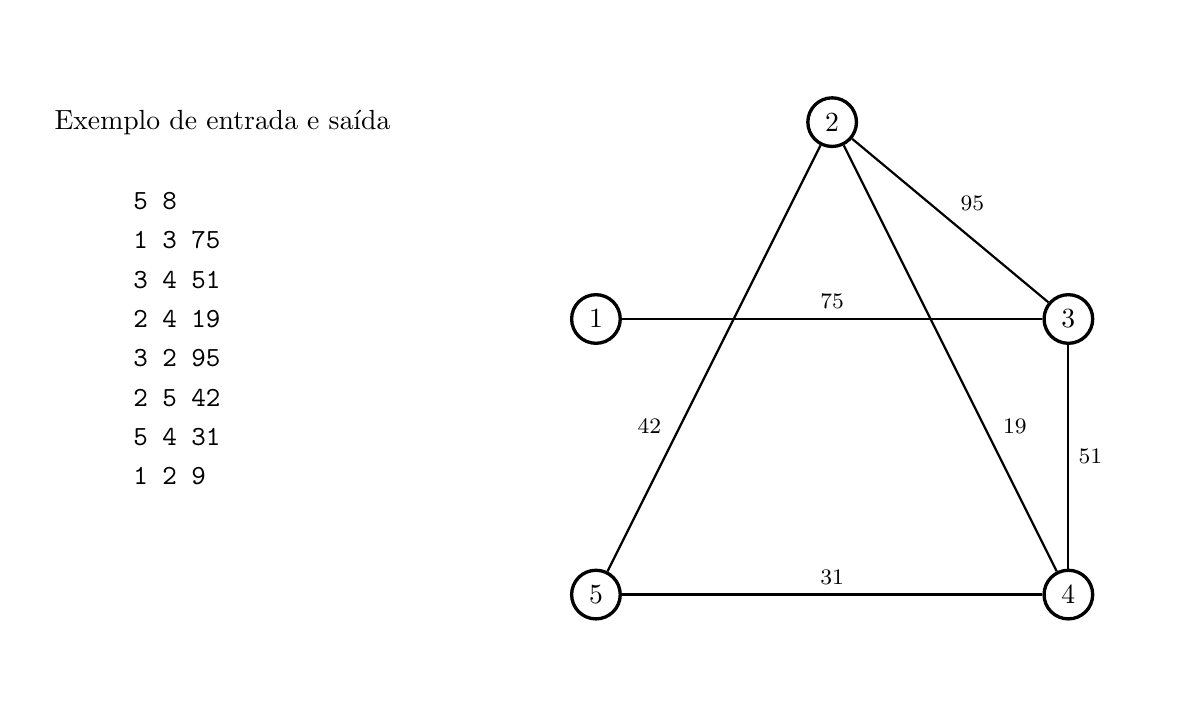
\begin{tikzpicture}
\node[draw,opacity=0] at (0, 0) {x};
\node[draw,opacity=0] at (14, 8) {x};

	\node[anchor=west] (header) at (0, 7.0) { \bbbold{Exemplo de entrada e saída} };


	\node[anchor=west] (line1) at (1.0, 6.0) { \bbtext{\texttt{5 8} } };








	\node[draw,very thick,circle] (node1) at (7.0, 4.5) { \bbtext{1} };

	\node[draw,very thick,circle] (node2) at (10.0, 7.0) { \bbtext{2} };

	\node[draw,very thick,circle] (node3) at (13.0, 4.5) { \bbtext{3} };

	\node[draw,very thick,circle] (node4) at (13.0, 1.0) { \bbtext{4} };

	\node[draw,very thick,circle] (node5) at (7.0, 1.0) { \bbtext{5} };


	\node[anchor=west] (line2) at (1.0, 5.5) { \bbtext{\texttt{1 3 75} } };












	\draw[thick](node1) to node[above] { \footnotesize \bbinfo{75} } (node3);


	\node[anchor=west] (line3) at (1.0, 5.0) { \bbtext{\texttt{3 4 51} } };


	\draw[thick](node3) to node[right] { \footnotesize \bbinfo{51} } (node4);


	\node[anchor=west] (line4) at (1.0, 4.5) { \bbtext{\texttt{2 4 19} } };


	\draw[thick](node2) to node[above right,pos=0.7] { \footnotesize \bbinfo{19} } (node4);


	\node[anchor=west] (line5) at (1.0, 4.0) { \bbtext{\texttt{3 2 95} } };


	\draw[thick](node3) to node[above right] { \footnotesize \bbinfo{95} } (node2);


	\node[anchor=west] (line6) at (1.0, 3.5) { \bbtext{\texttt{2 5 42} } };


	\draw[thick](node2) to node[above left,pos=0.7] { \footnotesize \bbinfo{42} } (node5);


	\node[anchor=west] (line7) at (1.0, 3.0) { \bbtext{\texttt{5 4 31} } };


	\draw[thick](node4) to node[above] { \footnotesize \bbinfo{31} } (node5);


	\node[anchor=west] (line8) at (1.0, 2.5) { \bbtext{\texttt{1 2 9} } };

\end{tikzpicture}
\end{frame}
\begin{frame}[plain,t]
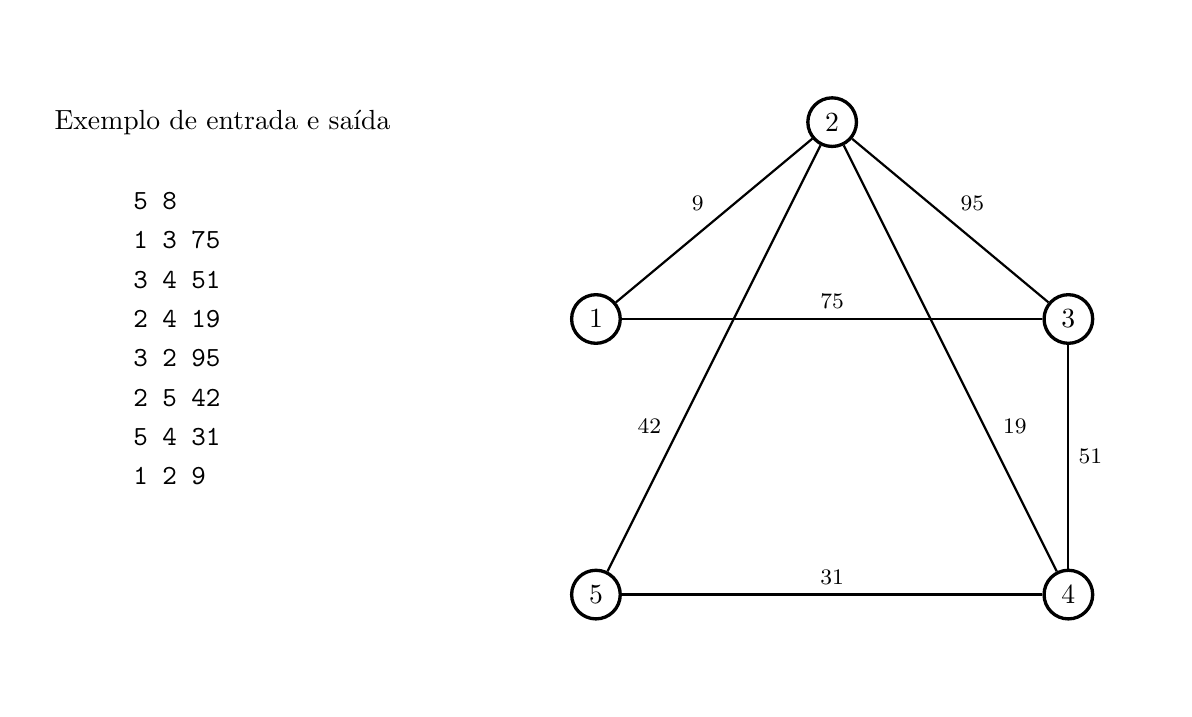
\begin{tikzpicture}
\node[draw,opacity=0] at (0, 0) {x};
\node[draw,opacity=0] at (14, 8) {x};

	\node[anchor=west] (header) at (0, 7.0) { \bbbold{Exemplo de entrada e saída} };


	\node[anchor=west] (line1) at (1.0, 6.0) { \bbtext{\texttt{5 8} } };








	\node[draw,very thick,circle] (node1) at (7.0, 4.5) { \bbtext{1} };

	\node[draw,very thick,circle] (node2) at (10.0, 7.0) { \bbtext{2} };

	\node[draw,very thick,circle] (node3) at (13.0, 4.5) { \bbtext{3} };

	\node[draw,very thick,circle] (node4) at (13.0, 1.0) { \bbtext{4} };

	\node[draw,very thick,circle] (node5) at (7.0, 1.0) { \bbtext{5} };


	\node[anchor=west] (line2) at (1.0, 5.5) { \bbtext{\texttt{1 3 75} } };












	\draw[thick](node1) to node[above] { \footnotesize \bbinfo{75} } (node3);


	\node[anchor=west] (line3) at (1.0, 5.0) { \bbtext{\texttt{3 4 51} } };


	\draw[thick](node3) to node[right] { \footnotesize \bbinfo{51} } (node4);


	\node[anchor=west] (line4) at (1.0, 4.5) { \bbtext{\texttt{2 4 19} } };


	\draw[thick](node2) to node[above right,pos=0.7] { \footnotesize \bbinfo{19} } (node4);


	\node[anchor=west] (line5) at (1.0, 4.0) { \bbtext{\texttt{3 2 95} } };


	\draw[thick](node3) to node[above right] { \footnotesize \bbinfo{95} } (node2);


	\node[anchor=west] (line6) at (1.0, 3.5) { \bbtext{\texttt{2 5 42} } };


	\draw[thick](node2) to node[above left,pos=0.7] { \footnotesize \bbinfo{42} } (node5);


	\node[anchor=west] (line7) at (1.0, 3.0) { \bbtext{\texttt{5 4 31} } };


	\draw[thick](node4) to node[above] { \footnotesize \bbinfo{31} } (node5);


	\node[anchor=west] (line8) at (1.0, 2.5) { \bbtext{\texttt{1 2 9} } };


	\draw[thick](node1) to node[above left] { \footnotesize \bbinfo{9} } (node2);

\end{tikzpicture}
\end{frame}
\begin{frame}[plain,t]
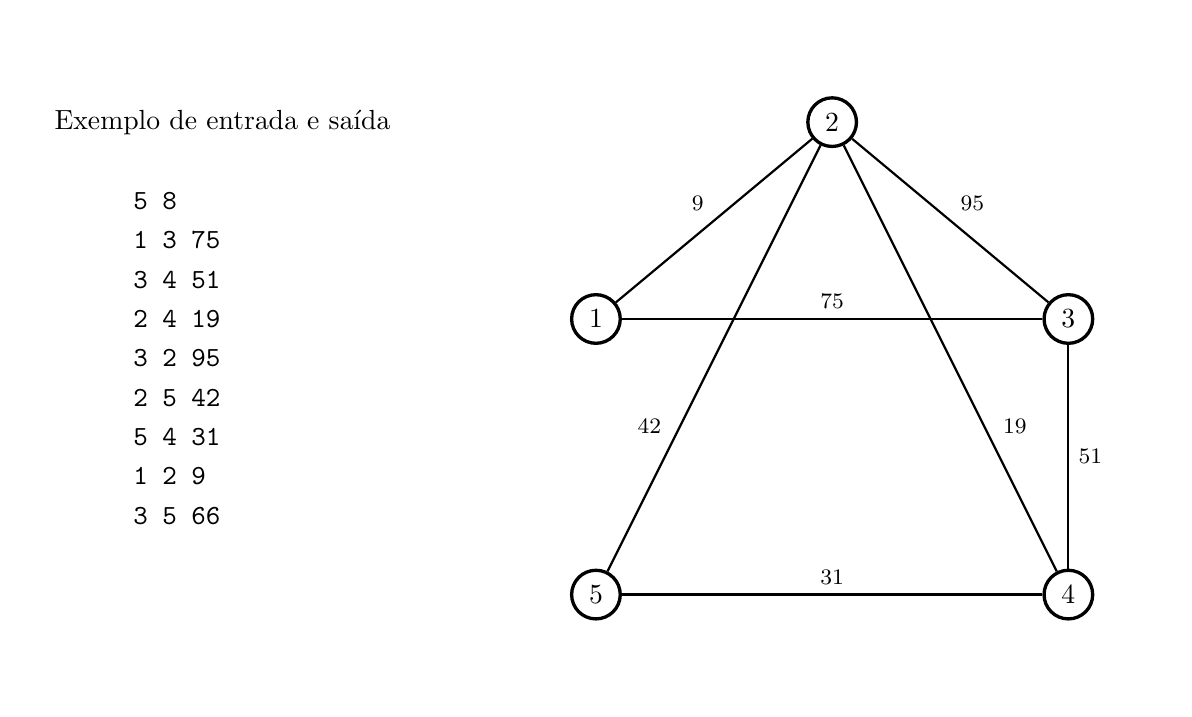
\begin{tikzpicture}
\node[draw,opacity=0] at (0, 0) {x};
\node[draw,opacity=0] at (14, 8) {x};

	\node[anchor=west] (header) at (0, 7.0) { \bbbold{Exemplo de entrada e saída} };


	\node[anchor=west] (line1) at (1.0, 6.0) { \bbtext{\texttt{5 8} } };








	\node[draw,very thick,circle] (node1) at (7.0, 4.5) { \bbtext{1} };

	\node[draw,very thick,circle] (node2) at (10.0, 7.0) { \bbtext{2} };

	\node[draw,very thick,circle] (node3) at (13.0, 4.5) { \bbtext{3} };

	\node[draw,very thick,circle] (node4) at (13.0, 1.0) { \bbtext{4} };

	\node[draw,very thick,circle] (node5) at (7.0, 1.0) { \bbtext{5} };


	\node[anchor=west] (line2) at (1.0, 5.5) { \bbtext{\texttt{1 3 75} } };












	\draw[thick](node1) to node[above] { \footnotesize \bbinfo{75} } (node3);


	\node[anchor=west] (line3) at (1.0, 5.0) { \bbtext{\texttt{3 4 51} } };


	\draw[thick](node3) to node[right] { \footnotesize \bbinfo{51} } (node4);


	\node[anchor=west] (line4) at (1.0, 4.5) { \bbtext{\texttt{2 4 19} } };


	\draw[thick](node2) to node[above right,pos=0.7] { \footnotesize \bbinfo{19} } (node4);


	\node[anchor=west] (line5) at (1.0, 4.0) { \bbtext{\texttt{3 2 95} } };


	\draw[thick](node3) to node[above right] { \footnotesize \bbinfo{95} } (node2);


	\node[anchor=west] (line6) at (1.0, 3.5) { \bbtext{\texttt{2 5 42} } };


	\draw[thick](node2) to node[above left,pos=0.7] { \footnotesize \bbinfo{42} } (node5);


	\node[anchor=west] (line7) at (1.0, 3.0) { \bbtext{\texttt{5 4 31} } };


	\draw[thick](node4) to node[above] { \footnotesize \bbinfo{31} } (node5);


	\node[anchor=west] (line8) at (1.0, 2.5) { \bbtext{\texttt{1 2 9} } };


	\draw[thick](node1) to node[above left] { \footnotesize \bbinfo{9} } (node2);


	\node[anchor=west] (line9) at (1.0, 2.0) { \bbtext{\texttt{3 5 66} } };

\end{tikzpicture}
\end{frame}
\begin{frame}[plain,t]
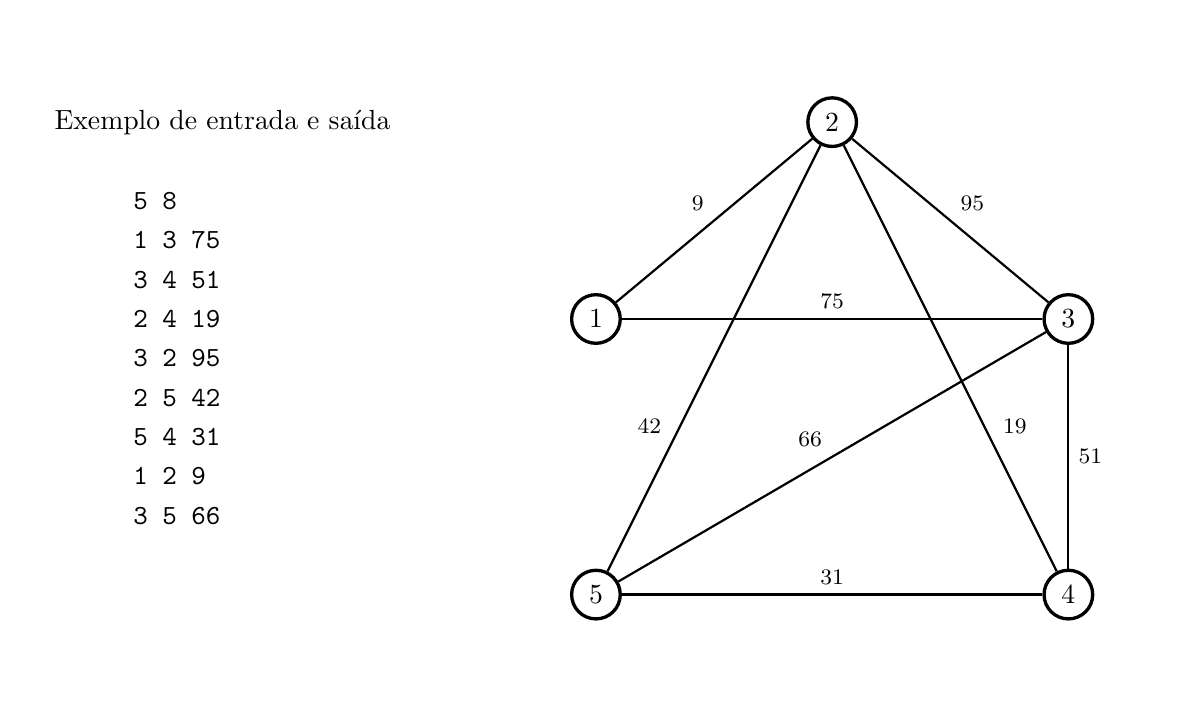
\begin{tikzpicture}
\node[draw,opacity=0] at (0, 0) {x};
\node[draw,opacity=0] at (14, 8) {x};

	\node[anchor=west] (header) at (0, 7.0) { \bbbold{Exemplo de entrada e saída} };


	\node[anchor=west] (line1) at (1.0, 6.0) { \bbtext{\texttt{5 8} } };








	\node[draw,very thick,circle] (node1) at (7.0, 4.5) { \bbtext{1} };

	\node[draw,very thick,circle] (node2) at (10.0, 7.0) { \bbtext{2} };

	\node[draw,very thick,circle] (node3) at (13.0, 4.5) { \bbtext{3} };

	\node[draw,very thick,circle] (node4) at (13.0, 1.0) { \bbtext{4} };

	\node[draw,very thick,circle] (node5) at (7.0, 1.0) { \bbtext{5} };


	\node[anchor=west] (line2) at (1.0, 5.5) { \bbtext{\texttt{1 3 75} } };












	\draw[thick](node1) to node[above] { \footnotesize \bbinfo{75} } (node3);


	\node[anchor=west] (line3) at (1.0, 5.0) { \bbtext{\texttt{3 4 51} } };


	\draw[thick](node3) to node[right] { \footnotesize \bbinfo{51} } (node4);


	\node[anchor=west] (line4) at (1.0, 4.5) { \bbtext{\texttt{2 4 19} } };


	\draw[thick](node2) to node[above right,pos=0.7] { \footnotesize \bbinfo{19} } (node4);


	\node[anchor=west] (line5) at (1.0, 4.0) { \bbtext{\texttt{3 2 95} } };


	\draw[thick](node3) to node[above right] { \footnotesize \bbinfo{95} } (node2);


	\node[anchor=west] (line6) at (1.0, 3.5) { \bbtext{\texttt{2 5 42} } };


	\draw[thick](node2) to node[above left,pos=0.7] { \footnotesize \bbinfo{42} } (node5);


	\node[anchor=west] (line7) at (1.0, 3.0) { \bbtext{\texttt{5 4 31} } };


	\draw[thick](node4) to node[above] { \footnotesize \bbinfo{31} } (node5);


	\node[anchor=west] (line8) at (1.0, 2.5) { \bbtext{\texttt{1 2 9} } };


	\draw[thick](node1) to node[above left] { \footnotesize \bbinfo{9} } (node2);


	\node[anchor=west] (line9) at (1.0, 2.0) { \bbtext{\texttt{3 5 66} } };


	\draw[thick](node3) to node[above left] { \footnotesize \bbinfo{66} } (node5);

\end{tikzpicture}
\end{frame}
\begin{frame}[plain,t]
\begin{tikzpicture}
\node[draw,opacity=0] at (0, 0) {x};
\node[draw,opacity=0] at (14, 8) {x};

	\node[anchor=west] (header) at (0, 7.0) { \bbbold{Exemplo de entrada e saída} };


	\node[anchor=west] (line1) at (1.0, 6.0) { \bbtext{\texttt{5 8} } };








	\node[draw,very thick,circle] (node1) at (7.0, 4.5) { \bbtext{1} };

	\node[draw,very thick,circle] (node2) at (10.0, 7.0) { \bbtext{2} };

	\node[draw,very thick,circle] (node3) at (13.0, 4.5) { \bbtext{3} };

	\node[draw,very thick,circle] (node4) at (13.0, 1.0) { \bbtext{4} };

	\node[draw,very thick,circle] (node5) at (7.0, 1.0) { \bbtext{5} };


	\node[anchor=west] (line2) at (1.0, 5.5) { \bbtext{\texttt{1 3 75} } };












	\draw[thick](node1) to node[above] { \footnotesize \bbinfo{75} } (node3);


	\node[anchor=west] (line3) at (1.0, 5.0) { \bbtext{\texttt{3 4 51} } };


	\draw[thick,color=BBCyan,dashed,very thick](node3) to node[right] { \footnotesize \bbinfo{51} } (node4);


	\node[anchor=west] (line4) at (1.0, 4.5) { \bbtext{\texttt{2 4 19} } };


	\draw[thick,color=BBCyan,dashed,very thick](node2) to node[above right,pos=0.7] { \footnotesize \bbinfo{19} } (node4);


	\node[anchor=west] (line5) at (1.0, 4.0) { \bbtext{\texttt{3 2 95} } };


	\draw[thick](node3) to node[above right] { \footnotesize \bbinfo{95} } (node2);


	\node[anchor=west] (line6) at (1.0, 3.5) { \bbtext{\texttt{2 5 42} } };


	\draw[thick](node2) to node[above left,pos=0.7] { \footnotesize \bbinfo{42} } (node5);


	\node[anchor=west] (line7) at (1.0, 3.0) { \bbtext{\texttt{5 4 31} } };


	\draw[thick,color=BBCyan,dashed,very thick](node4) to node[above] { \footnotesize \bbinfo{31} } (node5);


	\node[anchor=west] (line8) at (1.0, 2.5) { \bbtext{\texttt{1 2 9} } };


	\draw[thick,color=BBCyan,dashed,very thick](node1) to node[above left] { \footnotesize \bbinfo{9} } (node2);


	\node[anchor=west] (line9) at (1.0, 2.0) { \bbtext{\texttt{3 5 66} } };


	\draw[thick](node3) to node[above left] { \footnotesize \bbinfo{66} } (node5);


	\node[anchor=west] (info) at (7.0, 7.0) { \bbtext{MST} };





\end{tikzpicture}
\end{frame}
\begin{frame}[plain,t]
\begin{tikzpicture}
\node[draw,opacity=0] at (0, 0) {x};
\node[draw,opacity=0] at (14, 8) {x};

	\node[anchor=west] (header) at (0, 7.0) { \bbbold{Exemplo de entrada e saída} };


	\node[anchor=west] (line1) at (1.0, 6.0) { \bbtext{\texttt{5 8} } };








	\node[draw,very thick,circle] (node1) at (7.0, 4.5) { \bbtext{1} };

	\node[draw,very thick,circle] (node2) at (10.0, 7.0) { \bbtext{2} };

	\node[draw,very thick,circle] (node3) at (13.0, 4.5) { \bbtext{3} };

	\node[draw,very thick,circle] (node4) at (13.0, 1.0) { \bbtext{4} };

	\node[draw,very thick,circle] (node5) at (7.0, 1.0) { \bbtext{5} };


	\node[anchor=west] (line2) at (1.0, 5.5) { \bbtext{\texttt{1 3 75} } };












	\draw[thick](node1) to node[above] { \footnotesize \bbinfo{75} } (node3);


	\node[anchor=west] (line3) at (1.0, 5.0) { \bbtext{\texttt{3 4 51} } };


	\draw[thick,color=BBGreen,dashed,very thick](node3) to node[right] { \footnotesize \bbinfo{51} } (node4);


	\node[anchor=west] (line4) at (1.0, 4.5) { \bbtext{\texttt{2 4 19} } };


	\draw[thick,color=BBGreen,dashed,very thick](node2) to node[above right,pos=0.7] { \footnotesize \bbinfo{19} } (node4);


	\node[anchor=west] (line5) at (1.0, 4.0) { \bbtext{\texttt{3 2 95} } };


	\draw[thick](node3) to node[above right] { \footnotesize \bbinfo{95} } (node2);


	\node[anchor=west] (line6) at (1.0, 3.5) { \bbtext{\texttt{2 5 42} } };


	\draw[thick,color=BBGreen,dashed,very thick](node2) to node[above left,pos=0.7] { \footnotesize \bbinfo{42} } (node5);


	\node[anchor=west] (line7) at (1.0, 3.0) { \bbtext{\texttt{5 4 31} } };


	\draw[thick](node4) to node[above] { \footnotesize \bbinfo{31} } (node5);


	\node[anchor=west] (line8) at (1.0, 2.5) { \bbtext{\texttt{1 2 9} } };


	\draw[thick,color=BBGreen,dashed,very thick](node1) to node[above left] { \footnotesize \bbinfo{9} } (node2);


	\node[anchor=west] (line9) at (1.0, 2.0) { \bbtext{\texttt{3 5 66} } };


	\draw[thick](node3) to node[above left] { \footnotesize \bbinfo{66} } (node5);


	\node[anchor=west] (info) at (6.0, 7.0) { \bbtext{2$^a$ melhor MST} };










\end{tikzpicture}
\end{frame}
\begin{frame}[plain,t]
\begin{tikzpicture}
\node[draw,opacity=0] at (0, 0) {x};
\node[draw,opacity=0] at (14, 8) {x};

	\node[anchor=west] (header) at (0, 7.0) { \bbbold{Exemplo de entrada e saída} };


	\node[anchor=west] (line1) at (1.0, 6.0) { \bbtext{\texttt{5 8} } };


	\draw[->,color=BBBlack,very thick,-latex] (1.65, 1.75) to  (1.65, 0.75);

	\node[] (r) at (1.65, 0.5) { \bbinfo{110 121} };





	\node[draw,very thick,circle] (node1) at (7.0, 4.5) { \bbtext{1} };

	\node[draw,very thick,circle] (node2) at (10.0, 7.0) { \bbtext{2} };

	\node[draw,very thick,circle] (node3) at (13.0, 4.5) { \bbtext{3} };

	\node[draw,very thick,circle] (node4) at (13.0, 1.0) { \bbtext{4} };

	\node[draw,very thick,circle] (node5) at (7.0, 1.0) { \bbtext{5} };


	\node[anchor=west] (line2) at (1.0, 5.5) { \bbtext{\texttt{1 3 75} } };












	\draw[thick](node1) to node[above] { \footnotesize \bbinfo{75} } (node3);


	\node[anchor=west] (line3) at (1.0, 5.0) { \bbtext{\texttt{3 4 51} } };


	\draw[thick,color=BBGreen,dashed,very thick](node3) to node[right] { \footnotesize \bbinfo{51} } (node4);


	\node[anchor=west] (line4) at (1.0, 4.5) { \bbtext{\texttt{2 4 19} } };


	\draw[thick,color=BBGreen,dashed,very thick](node2) to node[above right,pos=0.7] { \footnotesize \bbinfo{19} } (node4);


	\node[anchor=west] (line5) at (1.0, 4.0) { \bbtext{\texttt{3 2 95} } };


	\draw[thick](node3) to node[above right] { \footnotesize \bbinfo{95} } (node2);


	\node[anchor=west] (line6) at (1.0, 3.5) { \bbtext{\texttt{2 5 42} } };


	\draw[thick,color=BBGreen,dashed,very thick](node2) to node[above left,pos=0.7] { \footnotesize \bbinfo{42} } (node5);


	\node[anchor=west] (line7) at (1.0, 3.0) { \bbtext{\texttt{5 4 31} } };


	\draw[thick](node4) to node[above] { \footnotesize \bbinfo{31} } (node5);


	\node[anchor=west] (line8) at (1.0, 2.5) { \bbtext{\texttt{1 2 9} } };


	\draw[thick,color=BBGreen,dashed,very thick](node1) to node[above left] { \footnotesize \bbinfo{9} } (node2);


	\node[anchor=west] (line9) at (1.0, 2.0) { \bbtext{\texttt{3 5 66} } };


	\draw[thick](node3) to node[above left] { \footnotesize \bbinfo{66} } (node5);


	\node[anchor=west] (info) at (6.0, 7.0) { \bbtext{2$^a$ melhor MST} };














\end{tikzpicture}
\end{frame}
\begin{frame}[plain,t]
\begin{tikzpicture}
\node[draw,opacity=0] at (0, 0) {x};
\node[draw,opacity=0] at (14, 8) {x};

	\node[anchor=west] (header) at (0.0, 6.0) { \Large \bbbold{Solução} };

\end{tikzpicture}
\end{frame}
\begin{frame}[plain,t]
\begin{tikzpicture}
\node[draw,opacity=0] at (0, 0) {x};
\node[draw,opacity=0] at (14, 8) {x};

	\node[anchor=west] (header) at (0.0, 6.0) { \Large \bbbold{Solução} };


	\node[anchor=west] (a) at (1.0, 5.0) { $\star$ \bbtext{O problema consiste em determinar a segunda melhor MST} };

\end{tikzpicture}
\end{frame}
\begin{frame}[plain,t]
\begin{tikzpicture}
\node[draw,opacity=0] at (0, 0) {x};
\node[draw,opacity=0] at (14, 8) {x};

	\node[anchor=west] (header) at (0.0, 6.0) { \Large \bbbold{Solução} };


	\node[anchor=west] (a) at (1.0, 5.0) { $\star$ \bbtext{O problema consiste em determinar a segunda melhor MST} };


	\node[anchor=west] (b) at (1.0, 4.0) { $\star$ \bbtext{O texto do problema garante a existência desta segunda melhor MST} };

\end{tikzpicture}
\end{frame}
\begin{frame}[plain,t]
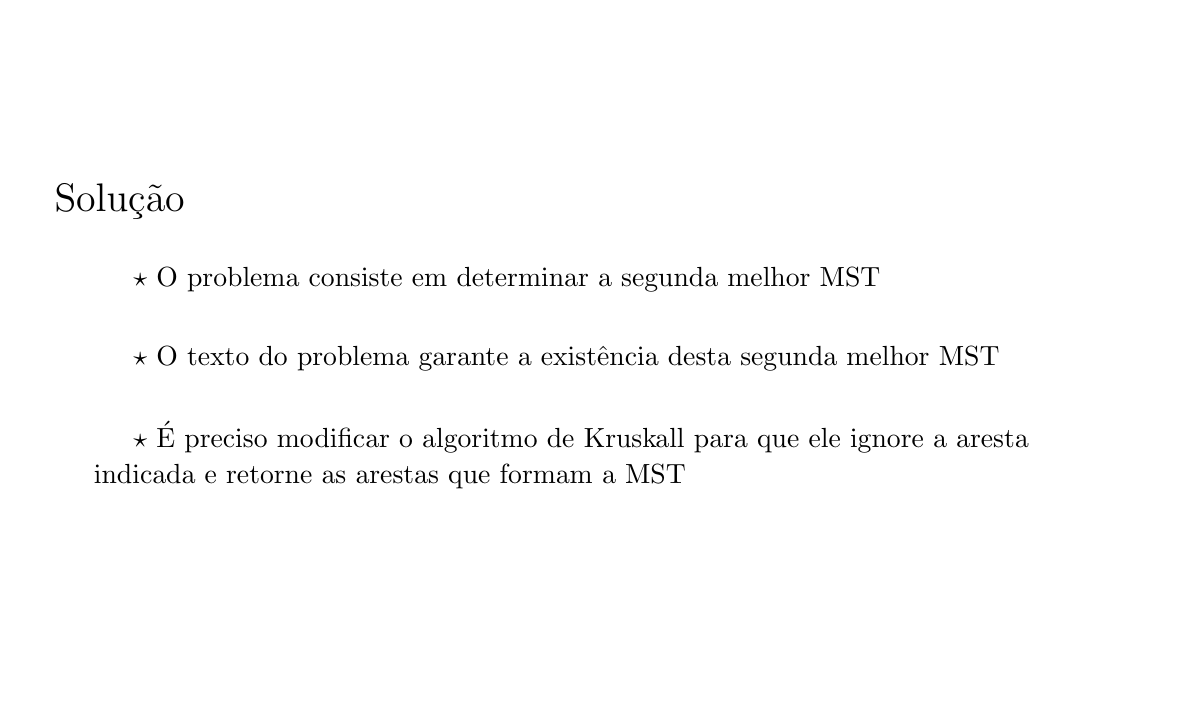
\begin{tikzpicture}
\node[draw,opacity=0] at (0, 0) {x};
\node[draw,opacity=0] at (14, 8) {x};

	\node[anchor=west] (header) at (0.0, 6.0) { \Large \bbbold{Solução} };


	\node[anchor=west] (a) at (1.0, 5.0) { $\star$ \bbtext{O problema consiste em determinar a segunda melhor MST} };


	\node[anchor=west] (b) at (1.0, 4.0) { $\star$ \bbtext{O texto do problema garante a existência desta segunda melhor MST} };


	\node[anchor=west] (c) at (1.0, 3.0) { $\star$ \bbtext{É preciso modificar o algoritmo de Kruskall para que ele ignore a aresta} };

	\node[anchor=west] (d1) at (0.5, 2.5) { \bbtext{indicada e retorne as arestas que formam a MST} };


\end{tikzpicture}
\end{frame}
\begin{frame}[plain,t]
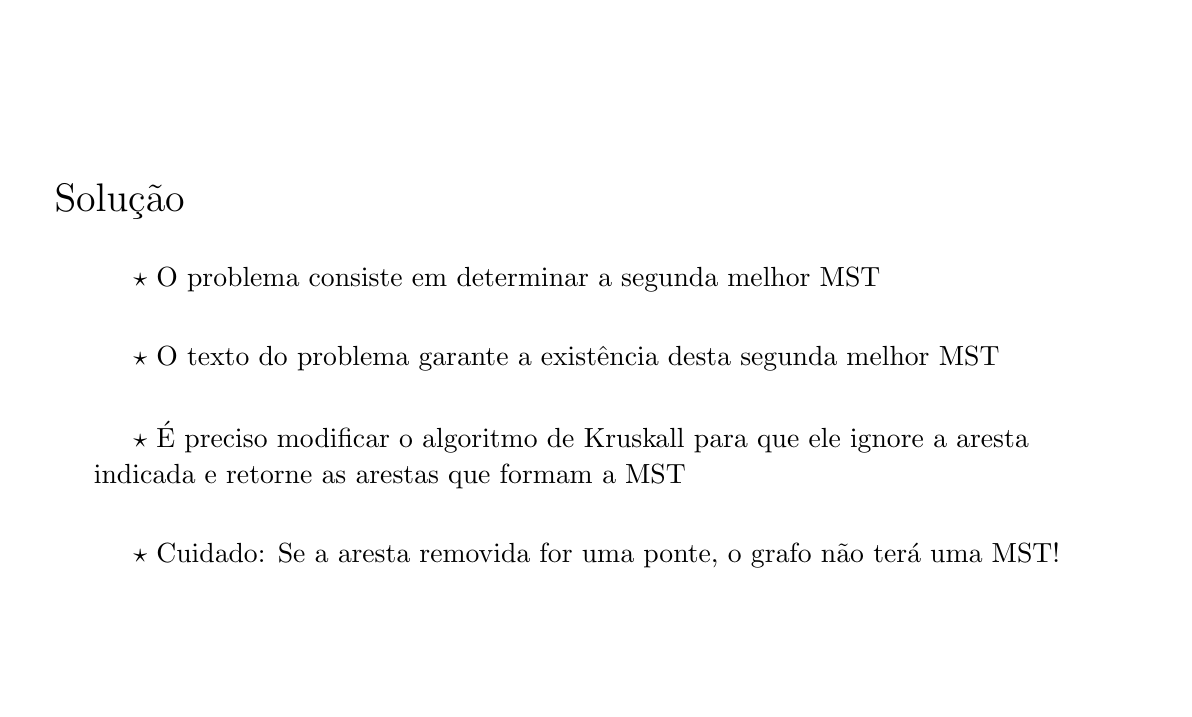
\begin{tikzpicture}
\node[draw,opacity=0] at (0, 0) {x};
\node[draw,opacity=0] at (14, 8) {x};

	\node[anchor=west] (header) at (0.0, 6.0) { \Large \bbbold{Solução} };


	\node[anchor=west] (a) at (1.0, 5.0) { $\star$ \bbtext{O problema consiste em determinar a segunda melhor MST} };


	\node[anchor=west] (b) at (1.0, 4.0) { $\star$ \bbtext{O texto do problema garante a existência desta segunda melhor MST} };


	\node[anchor=west] (c) at (1.0, 3.0) { $\star$ \bbtext{É preciso modificar o algoritmo de Kruskall para que ele ignore a aresta} };

	\node[anchor=west] (d1) at (0.5, 2.5) { \bbtext{indicada e retorne as arestas que formam a MST} };



	\node[anchor=west] (d) at (1.0, 1.5) { $\star$ \bbbold{Cuidado:} \bbtext{Se a aresta removida for uma ponte, o grafo não terá uma MST!} };

\end{tikzpicture}
\end{frame}
\begin{frame}[plain,t]

\inputsnippet{cpp}{69}{83}{codes/10600.cpp}

\end{frame}
\begin{frame}[plain,t]

\inputsnippet{cpp}{48}{67}{codes/10600.cpp}

\end{frame}
\end{document}
